
\documentclass[12pt, a4paper]{report}
\usepackage{graphicx}
\usepackage{amsmath}
\usepackage{float}
\usepackage{listings}
\usepackage{lmodern}  % for bold teletype font
\usepackage{xcolor}   % for \textcolor



\title{\textbf{EE2703 : Applied Programming Lab \\ Assignment 3}} % Title

\author{Potta Muni Asheesh \\ EE19B048} % Author name

\date{\today} % Date for the report

\begin{document}	
\lstset{
  language=Python,
  basicstyle=\ttfamily,
  columns=fullflexible,
  frame=single,
  breaklines=true,
  postbreak=\mbox{\textcolor{red}{$\hookrightarrow$}\space},
}	
		
\maketitle % Insert the title, author and date
\section*{Aim}
 The aim of the assignment is to fit the given data into a given model using the \textbf{least squares method}.\\
 The given model is as follows
 \begin{equation*}
 	g(t;A,B) = AJ_{2}(t) + Bt
 \end{equation*}

\section*{Generating and visualing data}
 The data required is generated using the \textit{generate$\_$data.py} python script provide. The script, when run, creates a file named \textit{fitting.dat} which contains 10 columns. The first column is time and next 9 columns are the model function evaluated at the corresponding time value to which some noise $n(t)$ is added. Each of the 9 columns have different noise with standard deviation $\sigma$ varying from $10^{-3}$ to $10^{-1}$ uniformly spaced in log scale. The $A$ and $B$ values used are 1.05 and -0.105.\\
 So, the data given in the columns corresponds to the function
 \begin{equation*}
 f(t) = 1.05J_2(t)-0.105t+n(t)
 \end{equation*} \\
 The data loaded using the \texttt{loadtxt()} function available in \texttt{numpy}. This gives a 2D array with contents of the file. This array is transposed and stored as \texttt{data} to make the columns accessable easily.\\
 Here is a plot showing the given data which contains noise along with the true curve.
 \begin{figure}[H]
 \centering
	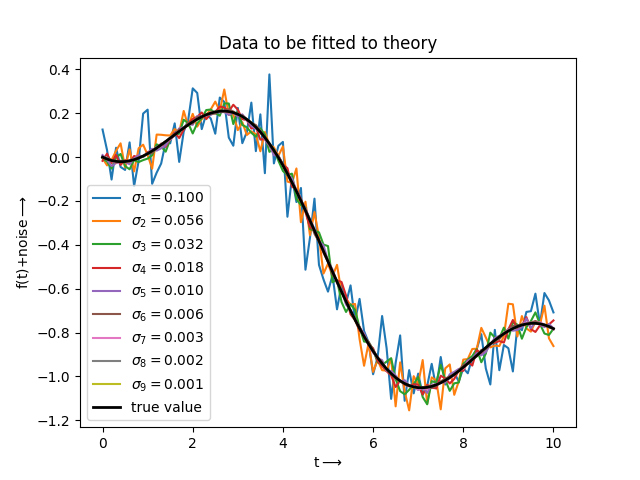
\includegraphics[scale=0.8]{Figure_1.png}  % Mention the image name within the curly braces. Image should be in the same folder as the tex file. 
	\caption{Plot of data from all columns}
	\label{fig1: Plot of data from all columns}
 \end{figure}
 
\section*{Visualing noise using errorbar}
 A convenient way of visualing nosie is to plot using errorbar. Python module  \texttt{matplotlib.pyplot} provides a function \texttt{errorbar()} which can be used to do this. The second column data is used for this. The standard deviation for noise in this data is $0.1$. This is how the plot looks like
 \begin{figure}[H]
 \centering
	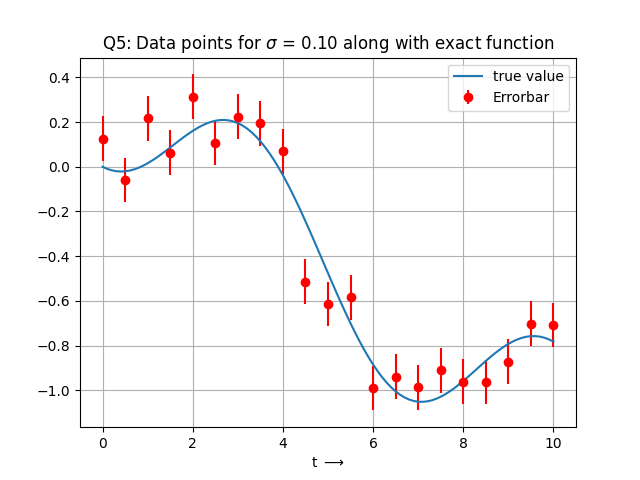
\includegraphics[scale=0.8]{Figure_2.png}  % Mention the image name within the curly braces. Image should be in the same folder as the tex file. 
	\caption{Errorbar plot}
	\label{fig2}
 \end{figure}
 These data points are the most problematic in predicting A and B values as they deviate the most from the true value.
 
\section*{Deducing A and B values using least squares}
 \subsection*{Matrix representation}
  The model $g(t;A,B)$ can be represented as a matrix equation as
  \begin{equation*}
  g(t;A,B) = \begin{bmatrix}
  J_2(t_1) & t_1 \\
  ... & ... \\
  J_2(t_m) & t_m
  \end{bmatrix} \begin{bmatrix}
  A \\
  B \\
\end{bmatrix}   \equiv M\cdot  p
  \end{equation*}
  The dot product $M \cdot p$ and the function $g(t;A,B)$ for the same values of $A$ and $B$. We can verify this plotting both the arrays on the same diagram.
  
  \begin{figure}[H]
 \centering
	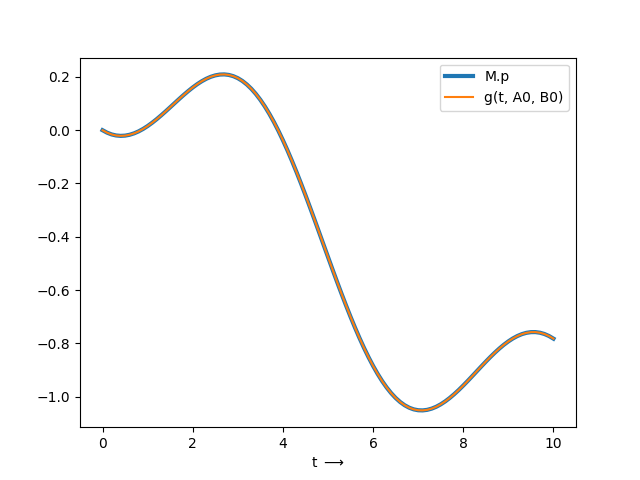
\includegraphics[scale=0.8]{Figure_3.png}  % Mention the image name within the curly braces. Image should be in the same folder as the tex file. 
	\caption{Verify the equivalence of $M \cdot p$ and $g(t;A,B)$}
	\label{fig3}
 \end{figure}
 
 \subsection*{Mean squared error}
 For $A_i = 0,0.1,..,2$ and $B_j = -0.2,-0.19,..,0$, we can use the data of columns 1 and 2 to compute the mean squared error $\epsilon_{ij}$ as
 
 \begin{equation*}
 \epsilon_{ij} = \frac{1}{101} \sum_{k=0}^{100} (f(t_k)-g(t_k;A_i,B_j))
 \end{equation*}
 
 Here, $\epsilon_{ij}$ is the value of mean squared error for corresponding values of $A_i$ and $B_j$. These values can be stored in a matrix. The matrix is created in python as follows
 
\begin{lstlisting}
A = np.linspace(0, 2, 21)
B = np.linspace(-0.2, 0, 21)
mean_squared_error = np.zeros((A.size, B.size))
for i in range(A.size):
   for j in range(B.size):
       mean_squared_error[i,j]+=(1/101)*(np.sum(np.square(data[1]-g(time,A[i],B[j]))))
\end{lstlisting}

 A contour plot of this matrix plotted using \texttt{contour()} function in \\ \texttt{matplotlib.pyplot}. The A and B values arrays along with the matrix created are given as parameters to this function as shown below. The plot looks as shown below (See Figure 4)
 
\begin{lstlisting}
f4, ax = plt.subplots()
CS = ax.contour(A, B, mean_squared_error, np.arange(0,1,0.025))
ax.clabel(CS, CS.levels[:5], inline=1, fontsize=10)
\end{lstlisting}

 \begin{figure}[H]
 \centering
	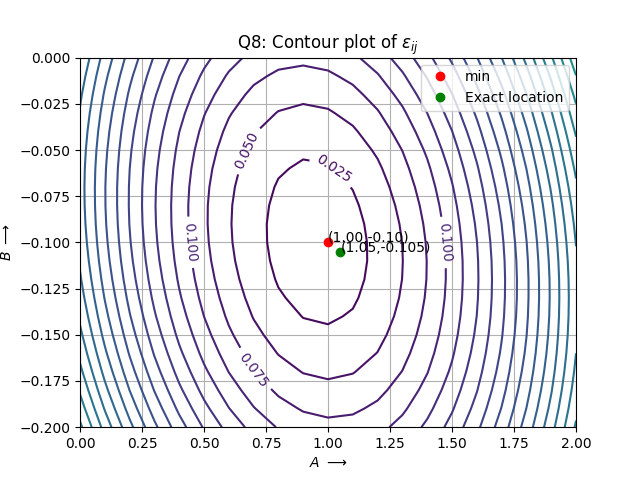
\includegraphics[scale=0.8]{Figure_4.png}  % Mention the image name within the curly braces. Image should be in the same folder as the tex file. 
	\caption{Contour plot}
	\label{fig4}
 \end{figure}
The index of minimum value in the matrix found using \\ \texttt{numpy.argmin()} which finds the index of minimum for the flattened matrix and \texttt{numpy.unravel\_index()} is used to find the index in original matrix. This can be done as follows
\begin{lstlisting}
min_error_i, min_error_j = np.unravel_index(mean_squared_error.argmin(), mean_squared_error.shape)
\end{lstlisting}
There is only one minimum in the plot which is at $(1.00,-0.105)$ whereas the actual values of $(A,B)$ are $(1.05,-0.105)$.

\subsection*{Least squares approximation}
 The matrix $M$ created above and column data $p$ can be passed to \texttt{lstsq()} function available in \texttt{scipy.linalg} to find the approximate values of $A$ and $B$ such that mean squared error is minimum. We can plot absolute difference of actual parameter value and approximated parameter value as Error against standard deviation of noise $\sigma_n$ for both A and B.
 \begin{figure}[H]
 \centering
	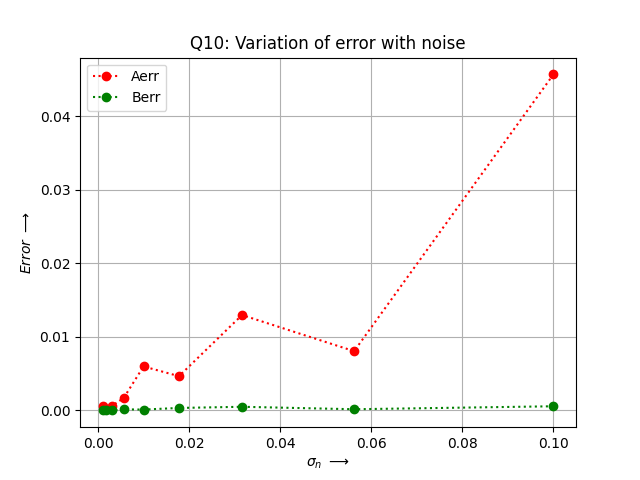
\includegraphics[scale=0.8]{Figure_5.png}  % Mention the image name within the curly braces. Image should be in the same folder as the tex file. 
	\caption{Error vs $\sigma_n$ (linear scale)}
	\label{fig5}
 \end{figure}
 The plot looks \textit{non-linear} in nature. When we plot both x-axis and y-axis in log scale, the plot looks roughly \textit{linear}. This tells us that error from actual value and $\sigma_n$ of noise are directly proportional.
 \begin{figure}[H]
 \centering
	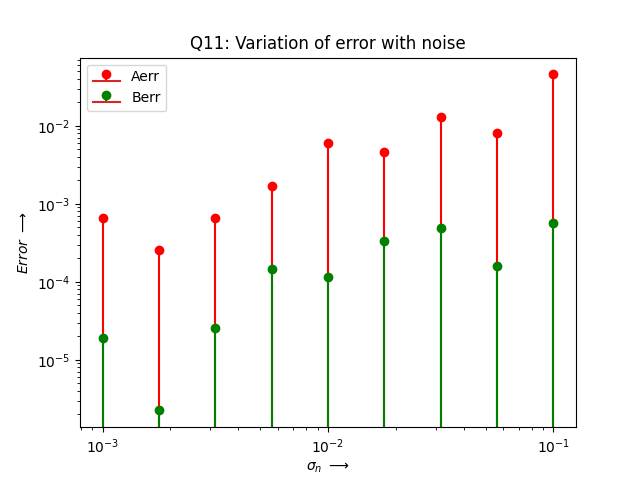
\includegraphics[scale=0.8]{Figure_6.png}  % Mention the image name within the curly braces. Image should be in the same folder as the tex file. 
	\caption{Error vs $\sigma_n$ (log scale)}
	\label{fig6}
 \end{figure}
   
\section*{Conclusion}
 For a given noisy data and model with parameters, we can approximate the parameters such that the mean squared error from actual model data is minimum using \textbf{least squares approximation method}. It was found that the standard deviation of noise is linearly related to error in parameter approximation in log scale.

\end{document}



 